\documentclass[10pt]{beamer}
\usefonttheme{serif}
\usetheme{Madrid}
% \usecolortheme{default}
\usecolortheme{beaver}
% \usecolortheme{crane}
\setbeamertemplate{navigation symbols}{}
\setbeamertemplate{footline}[frame number]
\usepackage{algorithm}
\usepackage{algpseudocode}
\usepackage{amsmath,amssymb,mathtools}

\title{Lab 3: Bayesian Learning and Boosting}
\author{Lucas Frykman}
\date{\today}

\begin{document}

\frame{\titlepage}

% --- SLIDE 1: INTRODUCTION & MAP ESTIMATES ---
\begin{frame}{Assignment 1 Bayesian Learning}
    \texttt{mlParams(X,labels)} outputs the following MLE estimate $\operatorname{argmax} p(\mu_k,\sigma_k|D_k)$ \\
    $$\mu_k = \frac{\sum_{i|c_i=k}x_i}{N_k}$$
    $$\Sigma_k = \frac{1}{N_k}\sum_{i|c_i=k} (x_i-\mu_k)^T(x_i-\mu_k)$$
    \centering
    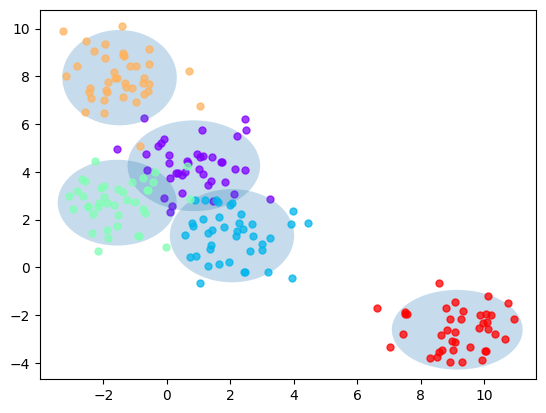
\includegraphics[width=0.6\textwidth]{image1.png}
\end{frame}
\begin{frame}{Assignment 2 Classification}
    \texttt{computePrior(X,labels)} outputs a \texttt{Cx1} array $p(k) \approx \frac{N_k}{N}$ \\
    \texttt{classifyBayes(X, prior, mu, sigma)} outputs a \texttt{Nx1} array of predictions $\operatorname{argmax}_k\delta_k(x)$ of test data $x$  \\
    where the discriminant is the log posterior $\delta_k(x) = \ln(p(k|x)) = -\frac{1}{2} \ln(|\Sigma_k|) - \frac{1}{2} (\mathbf{x}^* - \boldsymbol{\mu}_k) \Sigma_k^{-1} (\mathbf{x}^* - \boldsymbol{\mu}_k)^\top + \ln(p(k)) + C.$
\end{frame}
% --- SLIDE 2: ASSIGNMENT 3 - NAIVE BAYES ANALYSIS ---
\begin{frame}{Assignment 3: Naive Bayes Analysis}
    \begin{figure}
    \centering
    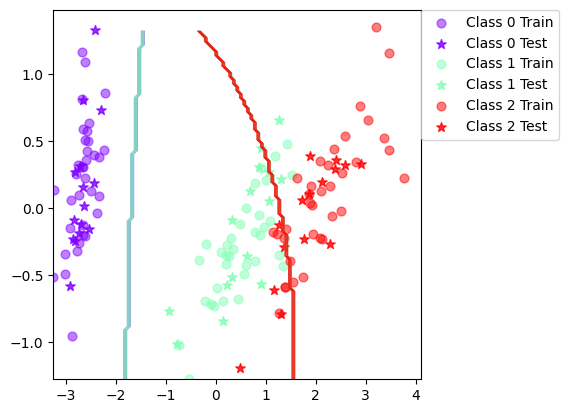
\includegraphics[width = 0.6\textwidth]{image2.png}
\end{figure} 
In the figure above illustrates the boundary lines $\{x : \delta_i(x) = \delta_j(x)\}$ \\ 
\texttt{Final mean classification accuracy:  89 with standard deviation 4.16}
\end{frame}
\begin{frame}{Assignment 3: Naive Bayes Analysis}
    \textbf{1. When can a feature independence assumption be reasonable and when not?} \\
    Reasonable when: 
    \begin{itemize}
        \item Physically independent features (eg: petal length and time of day)
        \item Limited training data: Using complex models that do not hold the independence assumption risk overfitting when learning feature dependencies
        \item When using a ranking based classifier like naive bayes. Ranking is maintained even if independence assumption is wrong.
    \end{itemize}
    Unreasonable when:
    Physically dependent features (eg: edjacent pixels on a image)
\end{frame}

\begin{frame}{Assignment 3: Naive Bayes Analysis}
    \textbf{2. how does the decision boundary look for the Iris dataset? How could one improve
the classification results for this scenario by changing classifier or, alternatively,
manipulating the data?}
    \begin{itemize}
        \item The decision boundary between class 0 and class 1 is straight due to large gap
        \item The decision boundary between class 1 and class 2 is curved and is underfit
        \item The data isn't uncorrelated (petal length and petal width tend to correlate well).
        \item Possible fix 1: use full bayes classification with full $\Sigma_k$ to allow Guassian distributions that tilt 
        \item  Possible fix 2: PCA can transform the data in to uncorrelated data before feeding in to naive bayes
        \item  Possible fix 3: Dimension reduction: multiply petal length and width together so you only have to classify based on one attribute
    \end{itemize}
\end{frame}
\begin{frame}{Assignment 4}
    Extend \texttt{mlParams} to \texttt{mlParams(X,labels,W)} that handles weighted instances
$$\mu_k = \frac{\sum_{\{i|c_i=k\}} \omega_i x_i}{\sum_{\{i|c_i=k\}} \omega_i}$$
$$\Sigma_k(m,m) = \frac{1}{\sum_{\{i|c_i=k\}} \omega_i} \sum_{\{i|c_i=k\}} \omega_i (x_i(m) - \mu_k(m))^2, m = 1,2...d$$
We're taking a weighted average. Some outliers in the training data need to have a bigger weight.
\end{frame}

% --- SLIDE 3: ASSIGNMENT 5 - BOOSTING BAYES ---
\begin{frame}{Assignment 5: Boosting the Bayes Classifier}
    \begin{itemize}
        \item Modify computePrior to \texttt{compurePrior(labels,W)} $p(k) = \frac{\sum_{i|c_i=k}w_i}{\sum w_i}$
        \item Implement Adaboost algorithm 
        \item Design functin classifyBoost(X, classifiers, alphas, Nclasses)
    \end{itemize}

    
\end{frame}
\begin{frame}{Assignment 5: Boosting the Bayes Classifier}
\begin{algorithmic}[1]
\State \textbf{Initialize} all weights uniformly: $\omega_i^1 = \frac{1}{N}$ for $i = 1, \dots, N$
\For{$t = 1, \dots, T$}
    \State Train weak learner using distribution $\omega^t$
    \State Get weak hypothesis $h^t$ and compute its error $\epsilon^t$ with respect to $\omega^t$:
    \[ \epsilon^t = \sum_{i=1}^N \omega_i^t (1 - \delta(h^t(x_i), c_i)) \]
    \State Choose the classifier vote weight $\alpha^t$:
    \[ \alpha^t = \frac{1}{2} \left( \ln(1 - \epsilon^t) - \ln(\epsilon^t) \right) \]
    \State Update the training instance weights:
    \[ \omega_i^{t+1} = \frac{\omega_i^t}{Z^t} \times 
    \begin{cases} 
      e^{-\alpha^t} & \text{if } h^t(x_i) = c_i \\ 
      e^{\alpha^t} & \text{if } h^t(x_i) \neq c_i 
    \end{cases} \]
    \Statex \textit{(where $Z^t$ is a normalization factor ensuring $\sum_i \omega_i^{t+1} = 1$)}
\State  Classifier: \[ H(x) = \arg\max_{c_i} \sum_{t=1}^T \alpha^t \delta(h^t(x), c_i) \]
\EndFor
\end{algorithmic}
\end{frame}
\begin{frame}{Assignment 5: Boosting the Bayes Classifier}
    \begin{figure}
        \centering
        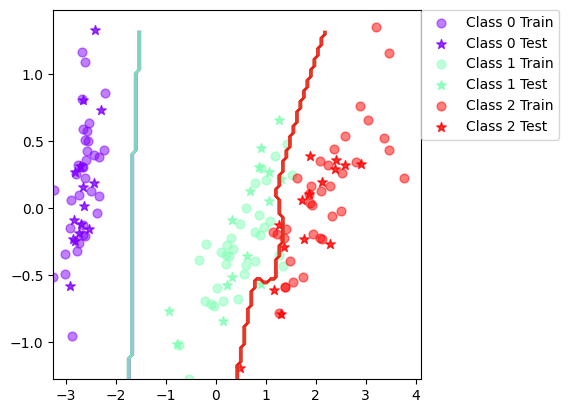
\includegraphics[width=0.6\textwidth]{image3.png}
        \label{Boosted bayes}
    \end{figure}
\end{frame}
\begin{frame}{Assignment 5: Boosting the Bayes Classifier}
\begin{table}[h!]
    \centering
    \begin{tabular}{|l|c|c|}
        \hline
        \textbf{Dataset} & \textbf{Basic Bayes} & \textbf{Boosted Bayes} \\ 
        \hline
        Iris & \texttt{Acc:89.0 std:4.16} & \texttt{Acc:94.7 std:2.82} \\ 
        \hline
        Vowels & \texttt{Acc:64.7 std:4.03} & \texttt{Acc:80.2  std:3.52} \\ 
        \hline
    \end{tabular}
    \vspace{0.2cm}
    \caption{Mean classification accuracy and standard deviation for the Basic and Boosted Bayes classifiers.}
    \label{tab:bayes_results}
\end{table}
    \textbf{1. Is there any improvement in classification accuracy? Why/why not?} \\

Yes, there is an improvement. 

This happens because the boosting algorithm actively re-weights misclassified examples 
so that they carry more importance in the next round (iteration t+1) of training. 
By doing this, the model is forced to focus harder on the difficult points and classify them correctly in subsequent runs
\end{frame}
\begin{frame}{Assignment 5: Boosting the Bayes Classifier}
    \textbf{2. Plot the decision boundary of the boosted classifier on iris and
compare it with that of the basic. What differences do you notice?
Is the boundary of the boosted version more complex?} 
\begin{itemize}
    \item Performance difference: The regular classifier incorrectly 
        classified some of the red and green data points, while the boosted version 
        successfully captured and classified them. This improvement is a direct result of the algorithm punishing those wrong classifications 
and increasing their weights.

    \item Yes the boosted bayes boundary is more complex and is wraps around specific training data. Bias has been decreased.
\end{itemize}

\end{frame}
\begin{frame}{Assignment 5: Boosting the Bayes Classifier}
\textbf{3. Can we make up for not using a more advanced model in the basic
classifier by using boosting?}
Yes, mostly. Boosting effectively compensates for a simple base classifier because the ensemble as a whole acts like a much more advanced and capable model.

The Catch: You have to be careful, as this increased complexity can easily cause the model to overfit the training data (and its noise), meaning boosting might not always be the best option depending on the dataset.
\end{frame}

% --- SLIDE 4: ASSIGNMENT 6 - DECISION TREES ---

\begin{frame}{Assignment 6: Decision Trees vs. Boosting}
    Decision tree boundary without boosting
    \begin{figure}
        \centering
        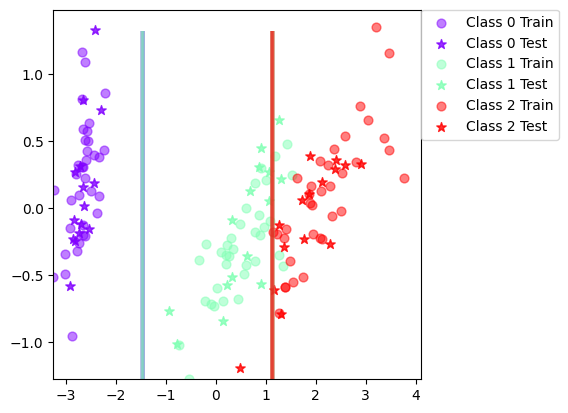
\includegraphics[width=0.6\textwidth]{image4.png}
    \end{figure}
\end{frame}

\begin{frame}{Assignment 6: Decision Trees vs. Boosting}
    Decision tree boundary with boosting
    \begin{figure}
        \centering
        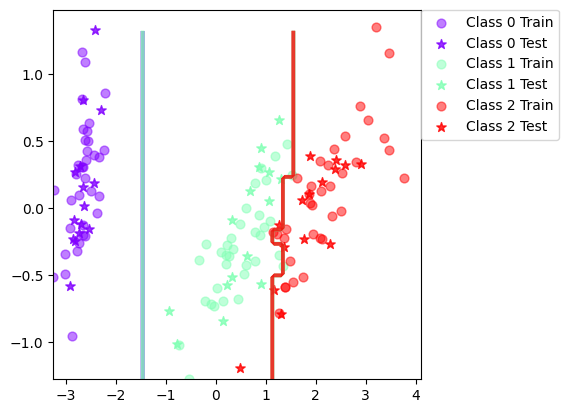
\includegraphics[width=0.6\textwidth]{image5.png}
    \end{figure}
\end{frame}

\begin{frame}{Assignment 6: Decision Trees vs. Boosting}
    \begin{table}[h!]
        \centering
        \begin{tabular}{|l|c|c|}
        \hline
        \textbf{Dataset} & \textbf{Basic Decision Tree} & \textbf{Boosted Decision Tree} \\ 
        \hline
        Iris & \texttt{Acc:92.4 std:3.67} & \texttt{Acc:94.6 std:3.67} \\ 
        \hline
        Vowels & \texttt{Acc:64.1 std:4.02} & \texttt{Acc:86.7 std:2.95} \\ 
        \hline
        \end{tabular}
        \vspace{0.2cm}
        \caption{Mean classification accuracy and standard deviation for the Basic and Boosted Decision Tree classifiers.}
    \end{table}
\end{frame}

\begin{frame}{Assignment 6: Decision Trees vs. Boosting}
\textbf{1. Is there any improvement in classification accuracy? Why/why not?} 

\begin{itemize}
    \item Yes this occours because Adaboost actively increases the weight of misclassified data points after every training round.
    \item The next classifier focuses entirely on the hardest examples correcting the ensembles previous mistakes
\end{itemize}
\end{frame}


\begin{frame}{Assignment 6: Decision Trees vs. Boosting}
\textbf{2. Plot the decision boundary of the boosted classifier on iris and
compare it with that of the basic. What differences do you notice?
Is the boundary of the boosted version more complex?} 
\begin{itemize}
    \item Yes the boosted decision boundary is more complex.
    \item The regular boundary misclassified some green points (higher bias)
    \item The boosted boundary bends to achieve both low training and test error (low variance and low bias)
\end{itemize}
\end{frame}

\begin{frame}{Assignment 6: Decision Trees vs. Boosting}
\textbf{3. Can we make up for not using a more advanced model in the basic
classifier by using boosting?}
Yes, because the boosting will act like a more advanced model, but it can cause
overfitting so it might not always be the best option.
\end{frame}

\begin{frame}{Assignment 7: Model Selection Criteria}
    Based on the lab criteria, here is how the classifiers compare
    \begin{itemize}
        \item \textbf{Outliers: } Decision Trees isolate outliers well. Naive Bayes means are easily skewed by them (if too little training data)
        \item \textbf{Irrelevant Inputs: } Trees perform inherent feature selection. Naive Bayes assumes all features are equally relevant
        \item \textbf{Predictive Power: } Boosted Trees typically offer the highest overall predictive accuracy
        \item \textbf{Mixed Data: } Trees handle categorical/mixed data natively. Gaussian Bayes requires continuous distributions
        \item \textbf{Scalability: } Naive Bayes scales exceptionally well with large dimensions ($D$) and instances ($N$). Trees become expensive as $D$ grows
    \end{itemize}
\end{frame}
% \begin{frame}{Assignment 7: Model Selection Criteria}
%     Naive Bayes
%     \begin{itemize}
%         \item \textbf{Outliers: } Performs badly with bad with extreme outliers (variance increases)
%         \item \textbf{Irrelevant Inputs: } Handles them relatively well. Suffers if irrelevant features highly correlated with relevant ones.
%         \item \textbf{Predictive Power: } Performs well but suffer with correlated data.
%         \item \textbf{Mixed Data: } Feature types need to be modeled with an appropiate distribution (eg: bernoulli or multinomial when categorical) guassian when continuous
%         \item \textbf{Scalability: } Computationally inexpensive. Can obtain values for large datasets.
%     \end{itemize}
% \end{frame}

\begin{frame}
    \begin{figure}
        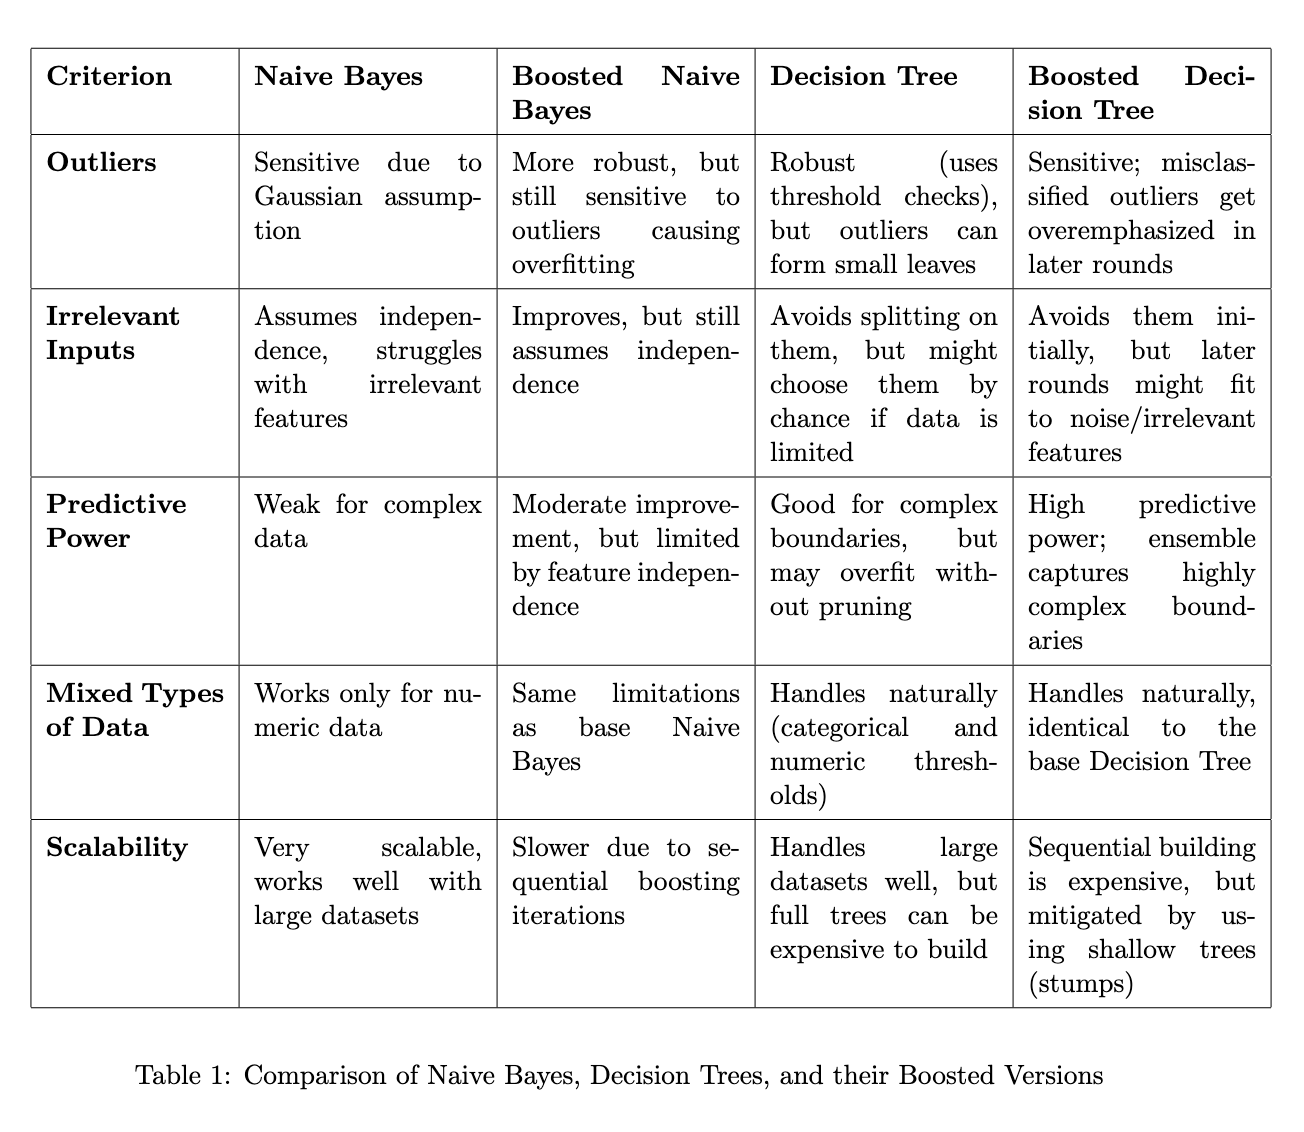
\includegraphics[width=0.8\textwidth]{table}
    \end{figure}
\end{frame}

\end{document}
